\documentclass[aspectratio=32]{beamer}


% Load packages
\usepackage{datetime}
\usepackage{graphicx}
\usepackage{amssymb}
\usepackage{longtable}
\usepackage{booktabs}
\usepackage{siunitx}
\usepackage{listings}
\usepackage{ifthen}
\usepackage{caption}
\usepackage{etoolbox}
\usepackage{hyperref}
\usepackage{ragged2e}
\usepackage{adjustbox}
\usepackage{xcolor}
\usepackage{float}
\usepackage[backend=biber, style=numeric]{biblatex}

% Metadata
\title{Mechanistic Interpretability on Irreducible Integers}
\date{\mydate\today}
\author{Noah Syrkis}

% BibTeX setup
\addbibresource{/Users/syrkis/code/press/library.bib}

% Listings and date setup
\newdateformat{mydate}{\monthname[\THEMONTH] \THEDAY, \THEYEAR}
% tight list
\providecommand{\tightlist}{\setlength{\itemsep}{0pt}\setlength{\parskip}{0pt}}

% Font setup
\usefonttheme{serif}
\renewcommand{\baselinestretch}{1.5}

% Text color setup
\setbeamercolor{normal text}{fg=black,bg=white}
\setbeamercolor{frametitle}{fg=black,bg=white}
\setbeamercolor{title}{fg=black,bg=white}
\setbeamercolor{bibliography entry author}{fg=black}
\setbeamercolor{bibliography entry title}{fg=black}
\setbeamercolor{bibliography entry location}{fg=black}
\setbeamercolor{bibliography entry note}{fg=black}
\setbeamercolor{bibliography entry journal}{fg=black}
\setbeamercolor{bibliography item}{fg=black}
\setbeamercolor{tableofcontents}{fg=black}
\setbeamercolor{section in toc}{fg=black}
\setbeamercolor{subsection in toc}{fg=black}
\setbeamercolor{itemize item}{fg=black}
\setbeamercolor{item}{fg=black}
\setbeamercolor{caption name}{fg=black}
\setbeamercolor{caption}{fg=black}

% Miscellaneous settings
\setbeamertemplate{frametitle continuation}[from second]
% section in toc number should be without dot after number
\setbeamertemplate{section in toc}{\inserttocsectionnumber{} \inserttocsection}
\setbeamertemplate{navigation symbols}{}
\setbeamertemplate{caption}[numbered]
\setbeamertemplate{headline}{}

% Footer setup
\setbeamertemplate{footline}
{
  \leavevmode
  \hbox{
    \ifnum\thepage>1
      \begin{beamercolorbox}[wd=\paperwidth,ht=2.5ex,dp=1ex]{page number}
        \hfill\insertpagenumber{} of \insertdocumentendpage\hspace{0.5cm}
        % \hfill\insertframenumber/\inserttotalframenumber\hspace{0.5cm}
      \end{beamercolorbox}
    \fi
  }
    \vspace*{0.5cm}
}

% Modify the frametitle template
\setbeamertemplate{frametitle}
{
  \vskip0.4cm
  \leavevmode
  \hbox{%
    \begin{beamercolorbox}[wd=\paperwidth,ht=0ex,dp=0ex]{frametitle}
      \hskip0.7cm\usebeamerfont{frametitle}%
        {\insertsectionnumber~\insertframetitle} % Otherwise, display the frame title with section number
    \end{beamercolorbox}
  }
}

% Custom title page
\defbeamertemplate*{title page}{customized}
{
  \begin{minipage}[c][\textheight][c]{0.55\textwidth}
    \begin{center}
      \usebeamerfont{title}\inserttitle\par
      \vspace{1cm}
      \small\usebeamerfont{author}\insertauthor\par
      \small\usebeamerfont{date}\insertdate\par
    \end{center}
  \end{minipage}%
  \hfill
  \begin{minipage}[c][0.7\textheight][c]{0.35\textwidth}
    \tableofcontents[hideallsubsections]
  \end{minipage}
}

\newlength{\maxwidth}
\setlength{\maxwidth}{.70\textwidth} % Example: 80% of the text width
\newlength{\maxheight}
\setlength{\maxheight}{.70\textheight} % Example: 70% of the text height
\setkeys{Gin}{width=\maxwidth,height=\maxheight,keepaspectratio}

\begin{document}

  % Front page
  \begin{frame}[allowframebreaks]
    \titlepage
  \end{frame}

  \section{\textbar{} Mech. interp. (MI)}\label{mech.-interp.-mi}

  \begin{frame}[allowframebreaks]{\textbar{} Mech. interp. (MI)}
  \begin{itemize}
  \tightlist
  \item
    Reverse-engineering neural network circuits.
  \item
    \textcite{nanda2023} shows MI modular addition transformer.
  \item
    There are (allegedly) low hanging fruits in MI.
  \end{itemize}
  \end{frame}

  \section{\textbar{} Grokking}\label{grokking}

  \begin{frame}[allowframebreaks]{\textbar{} Grokking}
  \begin{itemize}
  \tightlist
  \item
    Grokking is when a model suddenly generalises.
  \item
    \textcite{nanda2023} shows grokking in a transformer.
  \item
    Grokking means the weights represents an algorithm\ldots{}
  \item
    \ldots{} rather than a dataset.
  \end{itemize}

  \framebreak

  \begin{itemize}
  \tightlist
  \item
    Since MI is about reverse-engineering circuits\ldots{}
  \item
    \ldots{} grokking is a good sign for MI \ldots{}
  \item
    \ldots{} as it means circuits are \emph{there}.
  \end{itemize}
  \end{frame}

  \section{\texorpdfstring{\textbar{} \(\mathbb{Z}\)-sequences}{\textbar{} \textbackslash mathbb\{Z\}-sequences}}\label{mathbbz-sequences}

  \begin{frame}[allowframebreaks]{\textbar{} \(\mathbb{Z}\)-sequences}
  \begin{itemize}
  \tightlist
  \item
    \textcite{belcak2022} shows that transformers can sequences
    \(\in\mathbb{Z}\).
  \item
    They work in thousands of squences from OEIS \autocite{sloane2003}.
  \item
    They have four tasks: (1) sequence classification, (2) sequence
    comparission, (3) sequence continuation, and (4) sequence unmasking.
  \item
    Each task is strictly harder than the previous one.
  \end{itemize}

  \framebreak

  \begin{itemize}
  \tightlist
  \item
    Though \(\mathbb{Z}\)-sequences are simple to see, some can be hard
    to impossible to understand.
  \item
    \(1, 2, 3, ..., 100\) is easy, while the busy beaver sequence
    \autocite{aaronson2020} is hard/impossible.
  \item
    Complexity ranges from trivial to fuck-off-forever.
  \end{itemize}
  \end{frame}

  \section{\textbar{} MIII}\label{miii}

  \begin{frame}[allowframebreaks]{\textbar{} MIII}
  \begin{itemize}
  \tightlist
  \item
    MI on primes.
  \item
    Base 10 centric.
  \item
    Last digits \(d_l \in \{1,3,7,9\}\)
  \end{itemize}

  \framebreak

  \begin{longtable}[]{@{}llllrrrr@{}}
  \caption{Four digit dataset with numbers and labels
  (\([ \textbf{X} | \textbf{Y} ]\)).}\tabularnewline
  \toprule\noalign{}
  \(x_0\) & \(x_1\) & \(x_2\) & \(x_3\) & \(y_0\) & \(y_1\) & \(y_2\) &
  \(y_3\) \\
  \midrule\noalign{}
  \endfirsthead
  \toprule\noalign{}
  \(x_0\) & \(x_1\) & \(x_2\) & \(x_3\) & \(y_0\) & \(y_1\) & \(y_2\) &
  \(y_3\) \\
  \midrule\noalign{}
  \endhead
  1001 & 1003 & 1007 & 1009 & 0 & 0 & 0 & 1 \\
  1011 & 1013 & 1017 & 1019 & 0 & 1 & 0 & 1 \\
  \(\vdots\) & & & & & & & \(\vdots\) \\
  9981 & 9983 & 9987 & 9989 & 0 & 0 & 0 & 0 \\
  9991 & 9993 & 9997 & 9999 & 0 & 0 & 0 & 0 \\
  \bottomrule\noalign{}
  \end{longtable}

  \framebreak

  \begin{itemize}
  \tightlist
  \item
    I will focus on \textcite{he2023}'s simple transformer (see
    sec.~\ref{sec:simpletrans}).
  \item
    With possible expansion into spiking neural nets.
  \end{itemize}
  \end{frame}

  \section{\texorpdfstring{\textbar{} Simple trans.
  \autocite{he2023}}{\textbar{} Simple trans. {[}@he2023{]}}}\label{sec:simpletrans}

  \begin{frame}[allowframebreaks]{\textbar{} Simple trans. \autocite{he2023}}
  \begin{columns}[c]
  \begin{column}{0.48\textwidth}
  \begin{itemize}
  \tightlist
  \item
    Simple attention eq.~\ref{eq:attn}
  \end{itemize}
  \end{column}

  \begin{column}{0.48\textwidth}
  \begin{equation}\phantomsection\label{eq:attn}{\textbf{A}(\textbf{X}) \leftarrow (\alpha I_T + \beta \textbf{A}(\textbf{X}))}\end{equation}
  \end{column}
  \end{columns}

  \framebreak

  \begin{figure}
  \centering
  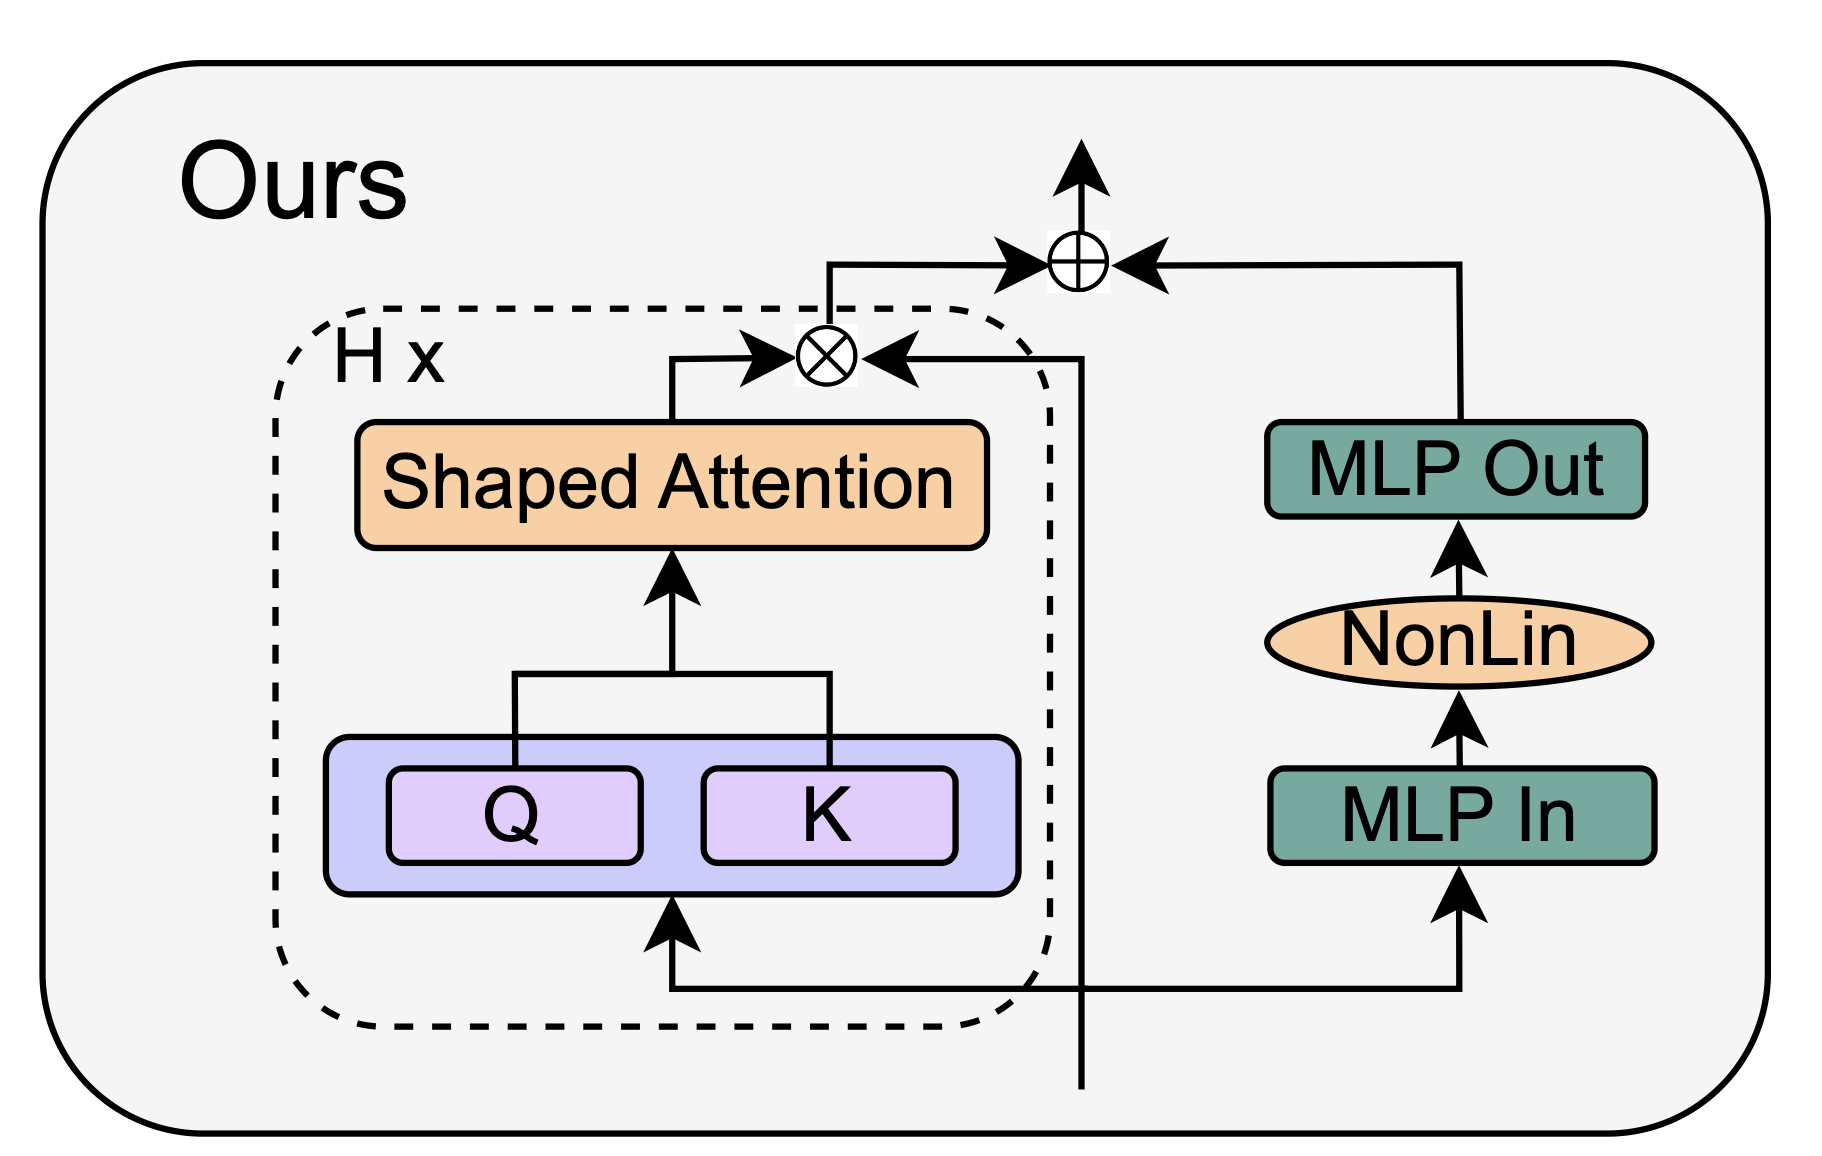
\includegraphics{attn.png}
  \caption{\textcite{he2023}'s transformer block}
  \end{figure}
  \end{frame}

  \section{\textbar{} Spiking NN}\label{spiking-nn}

  \begin{frame}[allowframebreaks]{\textbar{} Spiking NN}
  \begin{itemize}
  \tightlist
  \item
    I think spiking neural nets are cool.
  \item
    More brain like.
  \item
    Could be cool to do mech interp on them.
  \item
    See \textcite{olin-ammentorp2021} and \textcite{hu2014}
  \end{itemize}
  \end{frame}

  % bibliography
  
\begin{frame}[allowframebreaks]
  \Large{References}
  \small\linespread{1.2}\printbibliography
\end{frame}

\end{document}
